\documentclass[5p,authoryear]{elsarticle}
\makeatletter 
\def\ps@pprintTitle{%
 \let\@oddhead\@empty
 \let\@evenhead\@empty
 \let\@evenfoot\@oddfoot} % Supprimer le bas de page ELSEVIER
\makeatother
\usepackage[utf8]{inputenc} % En unicode
\usepackage[T1]{fontenc}
\usepackage[english]{babel}
\usepackage[babel=true]{csquotes} % permet de faire \enquote{a} (« a »)
\usepackage{amsmath} % pour certains signes mathématiques
\usepackage{amsthm} % Pour \begin{gather}
\usepackage{booktabs} % pour \toprule (un style de tableau)
\usepackage{multirow} % Pour colonnes multiples des tableaux
\usepackage{amssymb} % Pour \leqslant (<=, >=)
\usepackage{float}
\usepackage{hyperref} % 
\usepackage[english]{cleveref} 

% adding Code Blocking
\usepackage{listings}
\usepackage{color}

\definecolor{dkgreen}{rgb}{0,0.6,0}
\definecolor{gray}{rgb}{0.5,0.5,0.5}
\definecolor{mauve}{rgb}{0.58,0,0.82}

\lstset{frame=tb,
  language=Java,
  aboveskip=3mm,
  belowskip=3mm,
  showstringspaces=false,
  columns=flexible,
  basicstyle={\small\ttfamily},
  numbers=none,
  numberstyle=\tiny\color{gray},
  keywordstyle=\color{blue},
  commentstyle=\color{dkgreen},
  stringstyle=\color{mauve},
  breaklines=true,
  breakatwhitespace=true,
  tabsize=3
}




%\bibliographystyle{elsarticle-num}
\bibliographystyle{elsarticle-harv}

\usepackage{fancyhdr}
\pagestyle{fancy}
\lhead{MSDS 453 - SEC 56}
\rhead{Lee, J.}

\begin{document}

\begin{frontmatter}

\title{Clustering NBA News: \\Unsupervised Learning Methods}
\author{Jason Lee}
\address{Northwestern University, SPS \\Natural Language Processing \\2020SP MSDS 453-56}


\begin{abstract}
Information is power in the sports betting industry. 
With the amount of news articles and information hitting the internet daily, professional sports bettors need to organize and prioritize the incoming information in order to react with speed before market prices adjust.
As web scrapers scour the internet collecting NBA news articles, a document clustering algorithm is used to automatically sort these articles. 
The goal of this study is to utilize unsupervised learning methods to better understand and effectively sort the NBA news article corpus. There will be three overarching strategies to help with this goal: 1) Understand the corpus by using the articles as objects 2) Understand the corpus by using the terms in the articles as objects 3) Understand the corpus by topic modeling. 
\end{abstract}


\begin{keyword}
Natural Language Processing (NLP) \sep Clustering \sep Unsupervised Learning \sep NBA \sep Sports Betting 
\end{keyword}

\end{frontmatter}


\section{Introduction}\label{introduction}

The livelihoods of professional sports bettors revolve around staying current on all relevant sporting news. 
They must constantly be watching for breaking news alerts, injury updates, scores, and game specific analysis in order to execute advantageous investments.
As focused web crawlers scrape the internet capturing up-to-the-minute news on each team, there needs to be an automated process to organize the incoming information. 
This is exactly what unsupervised machine learning techniques, such as document clustering and topic modeling can do.

The document classification model created in the previous project required manual labeling of each document in order to properly train the classifier \citep{project2}. 
While the end result was effective, the manual labeling is an extremely tedious process absorbing a disproportionate quantity of valuable time that could be spent in more profitable areas. 
Unsupervised machine learning techniques provide an alternative route to solving the initial problem a sports bettor faces with overwhelming amounts of news articles.

Unsupervised learning algorithms do not need labels or user inputs to accomplish their goals.
They are able to read the incoming news articles and effectively sort them based on underlying similarities within the articles.
This automated sorting process, coupled with the focused web crawlers, will allow any sports bettor the ability to digest the right information in a timely manner. 

Building off of the corpus created by the focused web crawlers in the initial natural language processing (NLP) project \citep{project1} and the document vectors created in the previous project \citep{project2}, the purpose of this study is to utilize unsupervised learning methods to better understand and effectively sort the NBA news article corpus. 

There will be three means used to better understanding the corpus.

\begin{enumerate}
 \item Understand the corpus by using the articles as objects.
 \item Understand the corpus by using the words in the articles as objects.
 \item Understand the corpus by topic modeling. 
\end{enumerate} \\

There will also be nine specific activities, or tasks, carried out over the course of this study connected to these three different approaches. 


\subsection{Activities:}\label{activity}

The first activity prepares the NBA news article corpus. 
Activities 2-4 focus on understanding the corpus using the documents as objects, while activities 5-8 use the terms in the corpus as objects. 
The final activity uses topic modeling to try to further understand the corpus holistically.

\begin{enumerate}
 \item Activity 1: Upload the three vectorized document matrices of the NBA news article corpus for the Analyst Judgment, TF-IDF, and Doc2Vec Embedding vectorization methodologies and prepare them for the following unsupervised learning tasks.
 \item Activity 2: Perform partitioned cluster analysis (K-means) with the \textbf{documents as objects}. Utilize objective methods for determining the number of clusters (K). 
 \item Activity 3: Perform multidimensional scaling by way of the t-distributed stochastic neighbor embedding (t-SNE) algorithm with the \textbf{documents as objects}. Visualize the multidimensional scaling solutions in a two-dimensional space with clusters from Activity 2 as colors. 
 \item Activity 4: Analyze and compare the results from the multidimensional scaling and clustering techniques for the \textbf{documents} across the three different vectorization methodologies. Determine which of the three approaches provides the most clear-cut (interpretable) results.
 \item Activity 5: Perform multidimensional scaling by way of the t-distributed stochastic neighbor embedding (t-SNE) algorithm with the \textbf{terms as objects}. Visualize the multidimensional scaling solutions in a two-dimensional space with clusters as colors.
 \item Activity 6: Perform hierarchical cluster analysis with the \textbf{terms as objects}. Visualize the clustering solution with a dendrogram.
 \item Activity 7: Analyze and compare the results from the multidimensional scaling and clustering techniques in relation to the \textbf{terms} used in the corpus. Determine whether the Analyst Judgment or the TF-IDF document vectorization approach provides the most clear-cut (interpretable) results.
 \item Activity 8: Construct an ontology, or semantic network, of \textbf{terms} used in the corpus. 
 \item Activity 9: Perform topic modeling by using the Latent Dirichlet Allocation (LDA) algorithm.
\end{enumerate} \\

The completion of these activities will yield a comprehensive understanding of the NBA news article corpus and help create a finely tuned document clustering model.\\

A management problem addressed with this study is the high cost of time and resources needed to manually organize countless articles while searching for the right information that could provide an edge for a professional sports bettor. 
Another problem this project will solve is the speed to act on the new information before the markets have time to adjust. 

A document clustering model will be able to save a professional sports bettor countless hours by eliminating the manual effort needed to organize and read the various news articles and decide if it is useful or not. 

A.I. Sports is the financial sponsor for this study and the clustering and topic models built herein will be their property. These models will be implemented through their company to better server their professional sports betting clientele \citep{aisports}. 

There are three desired outcomes from this study: 
\begin{enumerate}
 \item Create a calibrated document clustering model.
 \item Determine whether using multidimensional scaling or clustering provides the most clear-cut results.
 \item Generate a reproducible Python notebook to easily share with colleagues. 
\end{enumerate} 


\section{Literature Review}\label{lit_rev}

Learning that takes place in nature by humans and animals can predominantly be categorized as unsupervised learning.
This learning comes about by naturally putting the pieces together from what is in view. 
Unsupervised learning algorithms are used to discover patterns within unlabeled datasets. 
Due to the unsupervised characteristic, the results may vastly differ from what a person might expect.
Yann LeCun, Chief A.I. Scientist at Facebook and recipient of the Turing Award for his work in Deep Learning, stated that the key step to attaining true A.I. is by solving the unsupervised learning problem \citep{handsOn}. 

Common machine learning approaches involve predicting a dependent variable based on its explanatory variables; this is called supervised learning. 
These algorithms learn by being fed lots of data with the dependent variable present. 
Unsupervised learning approaches are fed data with no dependent variable.
The algorithm tries to make sense of the data by grouping, or clustering, together items that have similar features.

Document clustering models are powerful natural language processing (NLP) unsupervised learning algorithms that enable automated sorting and filtering systems to function independently of human intervention \citep{Cookbook}. 
They are trained on a given corpus and are able to find similarities and dissimilarities between the individual documents \citep{handsOn}.
In production these document clustering models are able to ingest a new document and properly sort it into a category.


\subsection{Clustering Algorithms: K-Means}\label{kmeans}

The K-Means algorithm uses the nearest neighbor between the items and groups them together into (K) number of clusters.
The data scientist assigns the number of clusters to split the data into prior to training and then the K-Means algorithm will output a single cluster label for each item \citep{handsOn}.
The objective function when training a K-Means clustering model is to minimize the sum of the variations within each cluster \citep{handsOn}.
The algorithm strives to create roughly equal variations between the clusters during the training process \citep{Cookbook}.


There are three important assumptions made about the data if the desired outcome is to be reached when using the K-Means algorithm: 
\begin{enumerate}
 \item The clusters are convexly shaped.
 \item The features are all equally scaled.
 \item The number of observations are balanced between each group. 
\end{enumerate} \\

The K-Means algorithm is computationally expensive to train.
In order to speed up the training time, each item is randomly assigned a starting cluster, which is reassigned and updated during the training process until convergence is achieved \citep{handsOn}. 
When repeating the K-Means algorithm on the same dataset, the output of each iteration may be slightly different because of the randomly assigned starting cluster and setting a random seed is necessary to recreate the same results \citep{handsOn}. 


\subsubsection{Visualizing Clusters: t-SNE}\label{kmeans}

T-Distributed Stochastic Neighbor Embedding (t-SNE) is a process used to transform high-dimensional datasets into two or three dimensions allowing the data to be easily visualized \citep{handsOn}.  
T-SNE reduces the dimensionality in a nonlinear way that retains the meaning of the original data; this can be thought of as an encoder or an embedding \citep{lane}. 

Unlike some dimension reduction techniques, t-SNE's nonlinear transformations allow the local structure of the data to be retained, while simultaneously uncovering high-level global structures \citep{TSNE}. 
The newly created data points that are closer together in the two or three dimensional space are more similar, while the data points that are farther apart are dissimilar. 

A critique of the t-SNE algorithm is that there is no stable solution because of the nonconvex cost function \citep{handsOn}. 
This means that each initialization of the t-SNE algorithm on the same dataset will produce different results.
Setting a random seed is needed when using t-SNE for reproducibility purposes. 




\subsection{Clustering Algorithms: Hierarchical}\label{dendro}


There are two primary methods used when clustering in a hierarchical manner. 
The first methodology is a top-down approach using divisive clustering algorithms \citep{multivariate}.
The second methodology is a bottom-up approach using agglomerative clustering algorithms \citep{multivariate}.

In the agglomerative hierarchical clustering algorithm, each item begins as its own cluster and then is merged with similar items until the number of clusters remaining reaches the predetermined number of clusters, or a single cluster if no set number of clusters was designated \citep{Cookbook}. 

The divisive algorithm for hierarchical clustering starts with a single cluster containing every item in the dataset. 
A split in the data is then made creating two clusters. 
The divisive algorithm recursively splits the groups until each item is isolated in its own cluster \citep{multivariate}.

\subsubsection{Visualizing Clusters: Dendrogram}\label{Dendrogram}


Hierarchical clustering algorithm results can be viewed with a tree-based diagram called a dendrogram. 
The dendrogram allows for extremely easy interpretations of the complex underlying unsupervised learning algorithm.
Dendrograms use colors to represent clusters and lines to portray the relationships between items. 
The heights of the lines connecting items is representative of the similarity between them. 
Smaller heights correspond to strong similarities and taller heights correspond to less similarities between the items.

Figure \ref{dendro} is an example of how a hierarchical clustering model of varies U.S. cities is visualized with a dendrogram. 
There are four main clusters represented by the different colors. 
Beyond the obvious color coded clustering, the interpretation of this diagram is straight forward. 


\begin{figure}[!htb] \centering
	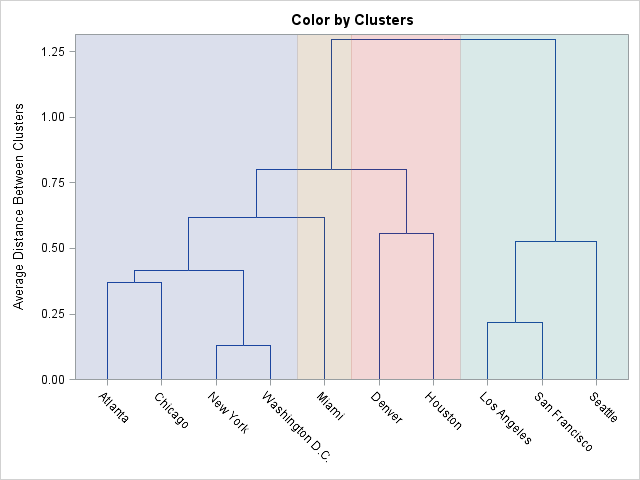
\includegraphics[width=3.4in]{figures/dendrogram_example.png}
	\caption[]{Example of a Dendrogram showing the hierarchical clustering of varies U.S. cities.} 
	\label{dendro} 
\end{figure}

In the blue cluster on the left, New York and Washington D.C. are connected by a very short line meaning the cities have strong similarities within this model.
Atlanta and Chicago are connected by a line that is just shorter than the line connecting them with New York and Washington D.C meaning they are slightly more similar than either city is with Washington D.C. or New York.

In the green cluster on the other side of the dendrogram, there is another short line connecting Los Angeles and San Francisco indicating strong similarities. 
The line connecting the green cluster containing west coast cities to the blue cluster containing east coast cities is the highest linkage in the diagram conveying the dissimilarity captured by the hierarchical clustering algorithm.


\subsection{Topic Modeling: LDA Models}\label{topic}

The Latent Dirichlet Allocation (LDA) model is a well established algorithm for topic modeling. 
This technique is able to determine which documents are most similar to each other by creating a simplified structure, or topic, within the raw text \citep{handsOn}.
These simplified structures, or topics, can be defined as collections of keywords that are representative and appear frequently within the given corpus \citep{sample-code2}. 
The topics found from LDA models help to quickly summarize and understand unstructured text documents \citep{handsOn}.

\clearpage

\section{Methodology}\label{meth}


The methodology implemented during this study is sequential progressing through completing each of the nine activities mentioned in Section \ref{activity} of the introduction. 


\subsection{Document Corpus}\label{corpus}

The corpus used in this study was collected by focused web crawlers, or Spiders. The Spiders were released onto each National Basketball Association (NBA) team's official website moving from page to page collecting six important pieces of information from every news article they came across.

\begin{enumerate}
 \item team  = The name of the NBA team
 \item url = The URL where the article is found
 \item tags = The topic tags for the article
 \item title = The title of the article
 \item date = The date the article was posted
 \item article = The complete news article
\end{enumerate} \\

The topics contained in this corpus are wide ranging. There are articles written about the team's humanitarian efforts, potential trades, pre-game/match-up analysis, injury updates, post-game analysis, deep dive player specific topics, player written articles, front office management news, team perception/fan sentiment, fan outreach, and miscellaneous articles.

This natural language processing (NLP) project is a continuation from the previous NLP project utilizing the matrices created from the three document vectorization approaches \citep{project2}. 

The three document vectorization approaches are as follows: 

\begin{enumerate}
 \item Analyst Judgment
 \item TF-IDF
 \item Neural Network Embedding
\end{enumerate} \\

Only the document vector with 300 dimensions for each approach will be used throughout this study.
There are 751 total NBA news articles in the corpus.


\subsection{Dependent Variable}\label{dependent}

While unsupervised machine learning algorithms do not need a dependent variable, A.I. Sports' goal with these models is to effectively filter and sort the NBA news articles in a way that adds value to professional sports bettors. 
The document clustering models built during this study will be partially evaluated based on how well they are able to differentiate between relevant and irrelevant news articles. The dependent variable is a binary flag. 

$$1 = Relevant$$
$$0 = Irrelevant$$

Topics that are included in the positive class include potential trades, pre-game/match-up analysis, injury updates, post-game analysis, and team perception/fan sentiment. Everything else will be contained in the negative, or Irrelevant, class.

Out of the 751 total news articles, 275 (36\%) articles are classified as relevant to a sports bettor and 476 articles are classified as irrelevant. 


\section{Computational Experiment and Results}

The entire Python code for this project will be attached to this paper, or can be reproduced by cloning the project's \href{https://colab.research.google.com/drive/13FXvFBOhEdyr4pE_DFnIXSTYEzwBTkV_?usp=sharing}{Google Colaboratory Notebook} at this url:

\begin{displayquote}
\centering
\href{https://colab.research.google.com/drive/13FXvFBOhEdyr4pE_DFnIXSTYEzwBTkV_?usp=sharing}{Google Colab Link}
\end{displayquote}

The Python script begins by uploading the previously processed NBA news article corpus, followed by nine activities.
Each activity is sectioned off in the notebook for ease of navigating. 
The Doc2Vec embedding vectorization method does not directly relate to specific terms the way that the Analyst Judgment and TF-IDF mothodologies do and will be disregarded in activities 5-8. 
The final activity does not use the document vectors and uses the raw text of each document in the corpus for topic modeling.

Activity 2 of the Python code is an adapted version of the cluster analysis example by Paul Huynh on the Reduced Reuters dataset \citep{sample-code1}. 
Activity 9 of the Python code is an adapted version of a topic modeling tutorial by Selva Prabhakaran using the Gensim library \citep{sample-code2}. 



\subsection{Activity 1: Vectorization}\label{one}

Each document in the corpus was converted to a vector of numeric values. 
The previous project created vector lengths of 50, 150, and 300 for each of the three vectorization methodologies \citep{project2}.
The vector length chosen for this study is 300 to provide the most depth and largest vocabulary for the clustering experiments that follow.

\subsubsection{Analyst Judgment Vectorization}\label{judge}

The Analyst Judgment methodology to vectorizing documents uses word statistics from the corpus. 
To easily generate the word statistics for this project, the CountVectorizer function from the SKLearn package in Python was used \citep{countVec}.
This function tokenizes the terms in the document and proceeds to count the number of times each token was used.


\subsubsection{TF-IDF Vectorization}\label{tfidf}

The Term Frequency-Inverse Document Frequency (TF-IDF) approach is similar to the analyst judgment, in that they both use word statistics from the corpus. 
For this study, the TfidfVectorizer function from the SKLearn package was used to calculate the TF-IDF values for each term in the corpus \citep{tfidf}. 


\subsubsection{Neural Network Embedding Vectorization}\label{exploration}

The final methodology to vectorizing the documents in the corpus is training a neural network embedding algorithm using Doc2Vec provided by way of the Gensim package in Python \citep{gensim}. 


\subsection{Activity 2: Clustering}\label{two}

The central goal in this activity is to understand the corpus by using the documents as objects. 
The vectors created in the previous activity were used as inputs into the clustering algorithms. 
After some experimenting, the number of clusters chosen for this and the next activity was six. 


\subsubsection{Analyst Judgment (K-Means)}\label{judge}

\begin{table}[!htb] 
  \centering 
  \begin{tabular}{@{\small}lllllll@{}} 
    \toprule % utilise booktabs
    & {\footnotesize C-1} &  {\footnotesize C-2} & {\footnotesize  C-3} & {\footnotesize  C-4} & {\footnotesize  C-5} & {\footnotesize  C-6} \\ \midrule
    Relevant & 117 & 118 & 0 & 5 & 0 & 35 \\
    Irrelevant & 118 & 315 & 1 & 32 & 1 & 9 \\
    Total & 235 & 433 & 1 & 37 & 1 & 44 \\
    \bottomrule
\end{tabular} \caption{NBA News Articles per Cluster for the Analyst Judgment vectorization methodology.} \label{table_eval}
\end{table}

The Analyst Judgment clusters were heavily skewed with the bulk of results residing in clusters 1 and 2. 
Cluster 3 and 5 each had only a single document classified. 

Cluster 6 proved to be the best cluster for a sports bettor to read containing 79.5\% relevant NBA news articles. 
Cluster 1 had 49.8\% relevant articles, which is a slight improvement from the initial 36.6\% distribution.


\subsubsection{TF-IDF (K-Means)}\label{tfidf}



\begin{table}[!htb] 
  \centering 
  \begin{tabular}{@{\small}lllllll@{}} 
    \toprule % utilise booktabs
    & {\footnotesize C-1} &  {\footnotesize C-2} & {\footnotesize  C-3} & {\footnotesize  C-4} & {\footnotesize  C-5} & {\footnotesize  C-6} \\ \midrule
    Relevant & 16 & 66 & 120 & 15 & 32 & 26 \\
    Irrelevant & 172 & 16 & 77 & 70 & 111 & 30 \\
    Total & 188 & 82 & 197 & 85 & 143 & 56 \\
    \bottomrule
\end{tabular} \caption{NBA News Articles per Cluster for the TF-IDF vectorization methodology.} \label{table_tfidf}
\end{table}


The document counts of the TF-IDF clusters were more evenly distributed across the six clusters compared to the other document vectorization methodologies. 
Table \ref{table_tfidf} provides the details for each cluster in this model.

Cluster 1 was able to filter down the relevant articles to only 8.5\% with a 188 sample size making it a valuable cluster to avoid for a sports bettor. 
Another cluster to avoid reading was cluster 4 containing only 17.6\% of its articles as relevant. 
Cluster 2 was able to peak at 80.5\% relevant news articles.
Cluster 3 contained the absolute maximum for relevant news articles with 120 making up 60.9\% of the total articles in the cluster.
Cluster 5 had 22.4\% relevant articles making it a decrease of 14.2\% from the original distribution and finally cluster 6 only had an increase of roughly 10\% coming in it at 46.4\% relevant.

Four of the six clusters in this model were able to create a sizeable lift discriminating between the relevant and irrelevant NBA news articles over the baseline 36.6\% relevant proportion. 


\subsubsection{Doc2Vec Embedding (K-Means)}\label{doc2}

\begin{table}[!htb] 
  \centering 
  \begin{tabular}{@{\small}lllllll@{}} 
    \toprule % utilise booktabs
    & {\footnotesize C-1} &  {\footnotesize C-2} & {\footnotesize  C-3} & {\footnotesize  C-4} & {\footnotesize  C-5} & {\footnotesize  C-6} \\ \midrule
    Relevant & 4 & 153 & 0 & 0 & 11 & 107 \\
    Irrelevant & 5 & 38 & 34 & 6 & 85 & 308 \\
    Total & 9 & 191 & 34 & 6 & 96 & 415 \\
    \bottomrule
\end{tabular} \caption{NBA News Articles per Cluster for the Doc2Vec Embedding vectorization methodology.} \label{table_eval}
\end{table}

Similar to the Analyst Judgment approach, the six clusters created with the Doc2Vec embedding vectors were heavily skewed with cluster 6 containing over half of the documents in the entire corpus. 
Clusters 1, 3, and 4 were left practically empty.

From a professional sports bettors perspective, this document clustering algorithm is not completely useless. 
Cluster 2 was able to group together 55.6\% of the entire relevant articles in the corpus. 
This cluster was made up of 80.1\% relevant articles with a sample size of 191 documents. 
Combining clusters 1, 3, 4, and 5 together, there are 145 documents and only 10.3\% are relevant to a sports bettor. 
These four clusters would make a reasonable filter to remove irrelevant news articles.

\subsection{Activity 3: Multidimensional Scaling (t-SNE)}\label{three}

Multidimensional Scaling was accomplished by using the t-distributed stochastic neighbor embedding (t-SNE) algorithm by way of the SKLearn package \citep{skTSNE} and visualized with the Yellowbrick library in Python \citep{Yellowbrick}.  


\subsubsection{Analyst Judgment (t-SNE)}\label{judge3}

Figure \ref{Analyst t-SNE} provides a two-dimensional visualization of the six clusters created from Activity 2 for the Analyst Judgement document vectorization methodology. 
As can be seen, the majority of the documents are spread out across the visual in the second cluster (light green) covering the upper left quarter of the graph or else in the first cluster (dark blue) covering the bottom right quarter of the graph. 

Cluster 6 (light blue) documents create a very tight cluster in the bottom right corner. 
These documents are predominately relevant to sports bettors and it is not surprising they create the most discernible cluster in the model.


The clustering results from this unsupervised learning model were not balanced creating very few distinguishable groupings in the t-SNE visualization. 



\begin{figure}[!htb] \centering
	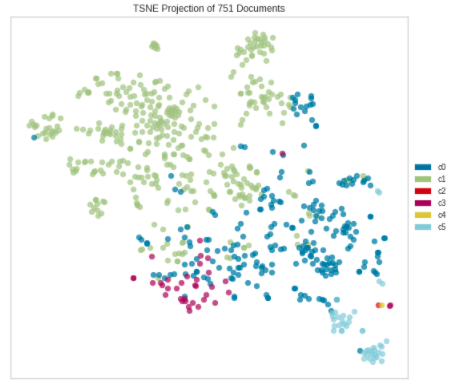
\includegraphics[width=3.4in]{figures/analyst_tsne.png}
	\caption[]{Analyst t-SNE} 
	\label{Analyst t-SNE} 
\end{figure}



\subsubsection{TF-IDF (t-SNE)}\label{tfidf3}


\begin{figure}[!htb] \centering
	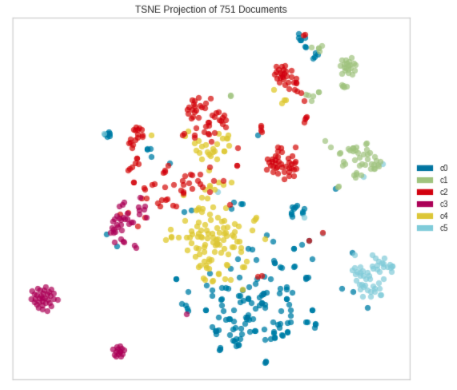
\includegraphics[width=3.4in]{figures/tfidf_tsne.png}
	\caption[]{TF-IDF t-SNE} 
	\label{TF-IDF t-SNE} 
\end{figure}

Figure \ref{TF-IDF t-SNE} provides the two-dimensional visualization of the six clusters created from Activity 2 for the TF-IDF document vectorization methodology.
Compared to the other two vectorization methodologies, the TF-IDF t-SNE visualization produces several tightly clustered documents signifying strong differences between the documents in the groupings.

Compared to the other two vectorization methodologies, the TF-IDF t-SNE visualization produces several tightly clustered documents signifying strong differences between the documents in the groups.
Cluster 2 ("c1" light green) and cluster 3 ("c2" red) in the upper right quarter are relevant articles with different topics creating several tight clusters.



\subsubsection{Doc2Vec Embedding (t-SNE)}\label{doc3}

\begin{figure}[!htb] \centering
	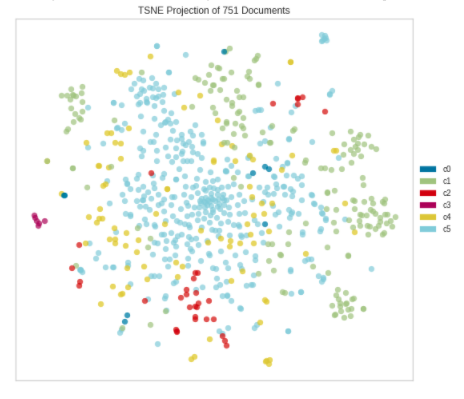
\includegraphics[width=3.4in]{figures/Doc2vec_tsne.png}
	\caption[]{Doc2Vec t-SNE} 
	\label{DocTSNE} 
\end{figure}

Figure \ref{DocTSNE} provides a two-dimensional visualization of the six clusters created from Activity 2 for the Doc2Vec embedding document vectorization methodology.

Cluster 2 ("c1" or the light green color) is interesting to note in this visualization. 
This cluster contains the majority of relevant news articles for a sports bettor.
These relevant articles cover several different topics like trades, pre-game analysis, post-game analysis, and team perception/sentiment.
There are several tight green clusters in various places around the outside perimeter of the visual.
Each of these tight circles represent the different topics that are all categorized as relevant news articles in the corpus.

\subsection{Activity 4: Comparison}\label{one}

The K-Means clustering algorithm and t-SNE visualization with the TF-IDF document vectors performed the best out of the three vectorization methodologies. 
There was clear discrimination between many of the clusters when using the TF-IDF vectors. 
The Doc2Vec and Analyst Judgment document vectors resulted in heavily skewed distributions of documents in the clusters. 
There was also very little discrimination between clusters when visualized with t-SNE.


Focusing on the professional sports bettor's problem to sort between the relevant and irrelevant news articles, the TF-IDF and the Doc2Vec clustering models both provide value.
The TF-IDF model was able to find value with each of the six clusters, extracting great value in four of the six clusters.
The Doc2Vec model was not able to discern value across all of the documents but the cluster 2 stuck out as a strong positive group.


\subsection{Activity 5: Terms t-SNE}\label{one}

The Doc2Vec embedding vectorization method does not directly relate to identifiable terms the way that the analyst judgment and TF-IDF mothodologies do and will be disregarded in Activity 5, 6, 7, and 8. 

The document vectors were transposed in order to use the terms as objects instead of the documents. 
This creates a matrix with 300 rows, one for each term, and 751 columns, one for each document.

\subsubsection{Analyst Judgment Terms (t-SNE)}\label{judge3}

Figure \ref{Analyst t-SNE2} provides a two-dimensional visualization of the ten clusters for the terms used by the Analyst Judgement vectorization methodology.
There are no tightly clustered groups in this model.

\begin{figure}[!htb] \centering
	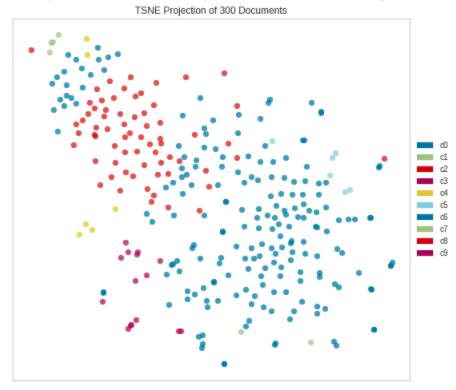
\includegraphics[width=3.4in]{figures/term_analyst_tsne.png}
	\caption[]{Analyst t-SNE} 
	\label{Analyst t-SNE2} 
\end{figure}

\subsubsection{TF-IDF Terms (t-SNE)}\label{tfidf3}

Figure \ref{TF-IDF t-SNE2} provides a two-dimensional visualization of the ten clusters for the terms used by the TF-IDF vectorization methodology.
There are no tightly clustered groups in this model.


\begin{figure}[!htb] \centering
	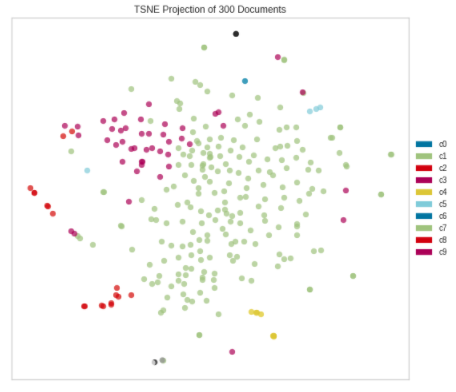
\includegraphics[width=3.4in]{figures/term_tfidf_tsne.png}
	\caption[]{TF-IDF t-SNE} 
	\label{TF-IDF t-SNE2} 
\end{figure}

\subsection{Activity 6: Hierarchical Clustering}\label{one}

The visuals for the Hierarchical clusters, both Analyst Judgment and TF-IDF, are difficult to view because of the size but are included the Appendix in Figure \ref{AnalystDendrogram} and \ref{TF-IDFDendrogram} respectively. 
An easier to read version is provided in the \href{https://colab.research.google.com/drive/13FXvFBOhEdyr4pE_DFnIXSTYEzwBTkV_?usp=sharing}{Google Colaboratory notebook} under the Activity 6 header. 

\subsubsection{Analyst Judgment}\label{judge3}

Hierarchical clustering using the vectors from the Analyst Judgment approach created three high-level clusters and sixteen clusters within a distance of 100. 
The dendrogram visualization in Figure \ref{AnalystDendrogram} shows these clusters.

The clustering and ordering of terms in this model make logical sense, for the most part.
Equivalence class terms were linked together with very short distances like "Lillard" and "Damian Lillard". 
Adjacent to Damian Lillard was his teammate McCollum.
Days of the week were also grouped right next to each other.

\subsubsection{TF-IDF}\label{tfidf3}

Hierarchical clustering using the vectors from the TF-IDF approach created seven high-level clusters and nineteen clusters within a distance of 3 (scaling is different than Analyst Judgment). 

It was promising seeing equivalence classes in the same clusters or very close together. 
"Trail blazers", "trail, "blazers", and "portland" are in their own black cluster.
Adjacent to this black cluster, a yellow cluster containing the terms "Atlanta", "hawks", and "Atlanta hawks".
Days of the week were right next to each other.
"Coach", "head", "Head Coach", and "players" were grouped together. 

The green cluster contained many of the key words in the relevant articles like "last night", "shoot" "three" "score" "rebound" "assist" "points" average point" "per game" and "win".
The red cluster was focused on words that had to do with community outreach and the family. 


\subsection{Activity 7: Comparison}\label{one}

The t-SNE methodology was much more difficult to interpret compared to the hierarchical clsutering methodology. 
It appeared as if there were not many distinct clusters for the terms in the corpus using the t-SNE method for both TF-IDF and Analyst Judgment vectors.
Compared to the documents as objects clustering t-SNE visualizations in Activity 4, the terms as objects clustering t-SNE visualizations do not provide much value when trying to understand the corpus deeper.

Using a dendrogram to visualize the hierarchical clusters created made for an extremely easy interpretation. 
The terms that were closer together had higher similarity metrics. 
Cleveland, Nuggets, Rockets, Houston, Clippers, and Lakers, were all right next to each other in the orange cluster in Figure \ref{AnalystDendrogram}, while Trail Blazers, Trail, Blazers, Portland, and Lillard were all close together in the sky blue cluster.

\subsection{Activity 8: Ontology}\label{one}

Figure \ref{Ontology} provides a high-level view of the terms in the NBA news article corpus relevant to a professional sports bettor. 
There are three categories that the NBA can be broken into from a sports betting perspective: Teams, Games, and Officials. 


\begin{figure}[!htb] \centering
	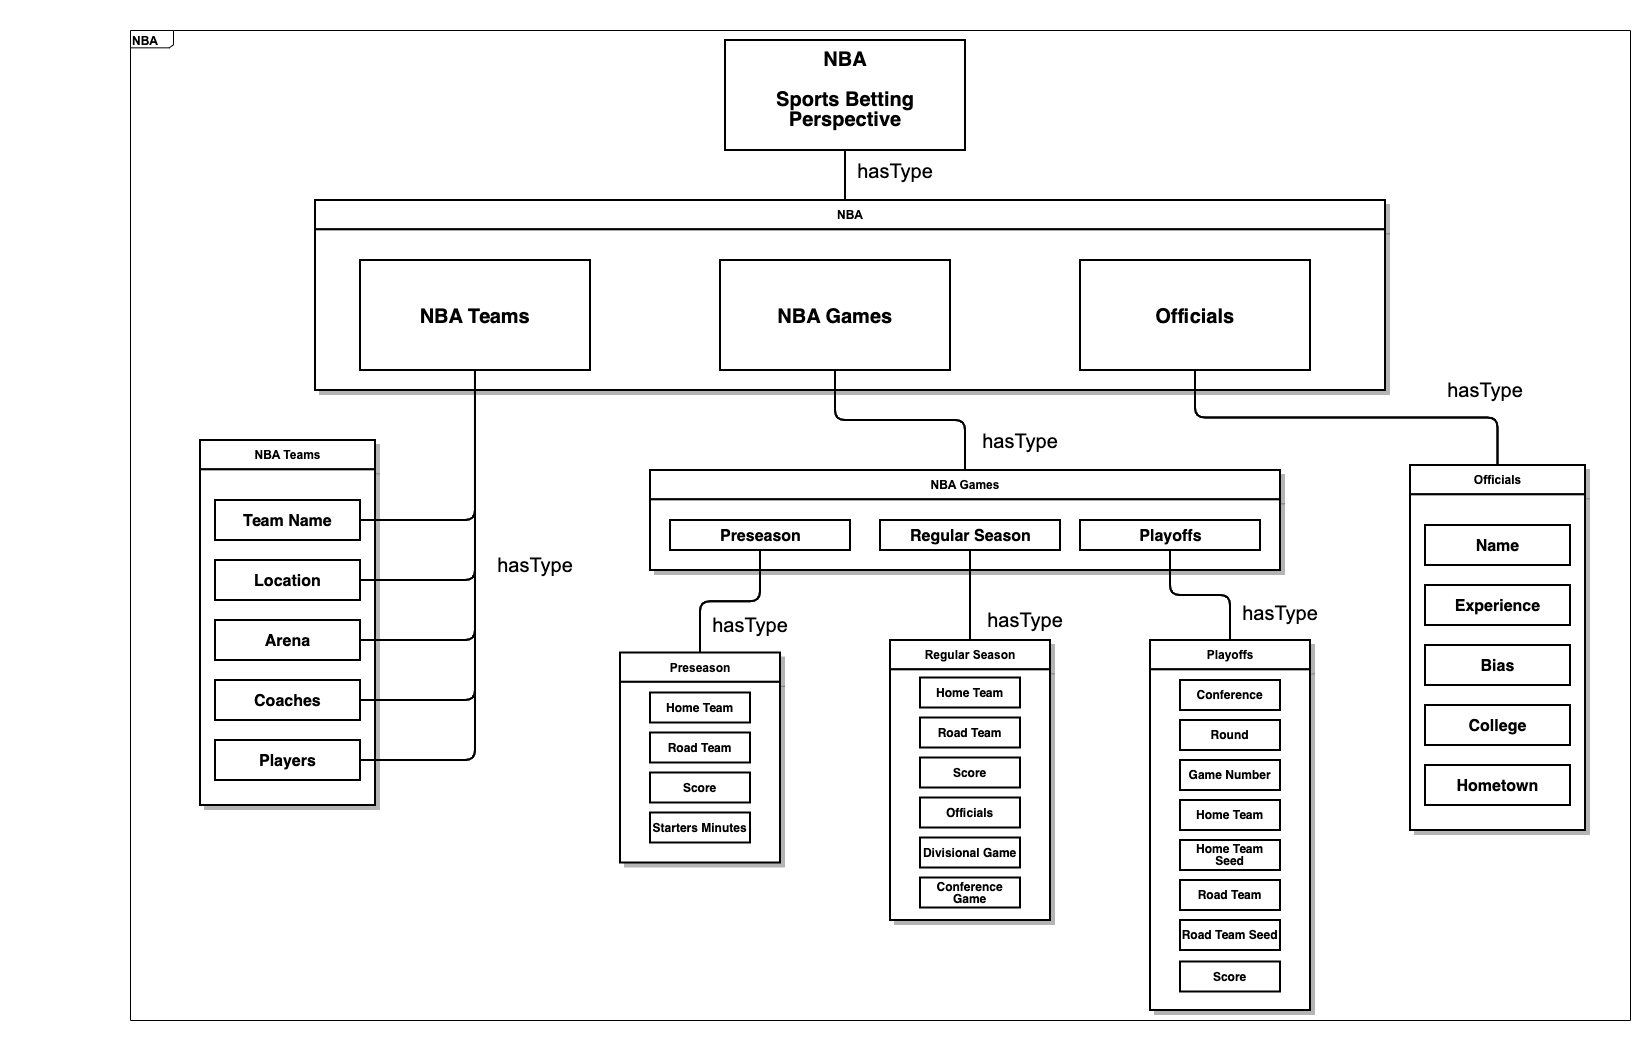
\includegraphics[width=3.7in]{figures/Ontology.png}
	\caption[]{Ontology for the NBA from a Sports Betting perspective} 
	\label{Ontology} 
\end{figure}

The Golden State Warriors will be used as an example for the NBA team node.
NBA teams are comprised of several elements. 
Each team has its name. 
Within the name category, there is the actual team name and various nicknames. 
"Golden State Warriors", "Golden State", "Warriors", "Dubs", "The Town" are five terms that an algorithm would view as different but one with domain knowledge understands they all represent the exact same thing. 
These terms should be grouped together into a single term to reduce the complexity and noise in the model.

Then each team has a Location. "City by the bay", "Golden State", "California", "San Francisco", "Oakland", "Bayside", "Dub Nation", "Mission Bay" are all terms that represent where the Golden State Warriors are located. Each team also has an arena. "Oakland Arena", "Oracle Arena", "Oracle", "Warriors Arena", and "Chase Center" all represent where the home games for the Warriors are played. The location of the team and the arena they play in for most purposes represent the exact same thing. Each of the 13 terms listed above could easily be grouped together into a single term further reducing the model complexity and removing unneeded noise.

Players and coaches are all people in different positions first and last names and most likely a nickname that are equivalence classes. 

From a high-level unsupervised document clustering modeling perspective, the various detailed terms listed above introduce too much noise in the data and should be condensed to the nodes presented in Figure \ref{Ontology}.



\subsection{Activity 9: Topic Modeling}\label{one}

Independent of the previous activities and the various document vectors, the topic modeling process is another unsupervised learning method used to understand and sort the various NBA news articles in the corpus.

The topic modeling algorithm was fed unigrams, bigrams, and trigrams creating thousands of possible terms to learn from.
There were \footnotemark{four} unique topics created by using the LDA algorithm.
Figure \ref{cloud} provides a word cloud for each topic created in this activity giving a better idea on the types of words in each topic.


\footnotetext{Python is a base 0 language meaning that 0 is the first term, which could make some of the visuals confusing. "Topic 0" is the first topic, while "Topic 3" is the fourth and final topic created in this activity.}



\begin{figure}[!htb] \centering
	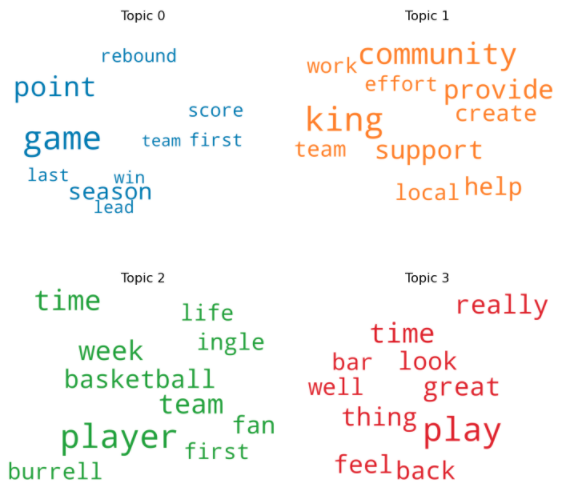
\includegraphics[width=3.4in]{figures/word_cloud.png}
	\caption[]{Topic Word Count} 
	\label{cloud} 
\end{figure}



\begin{figure}[!htb] \centering
	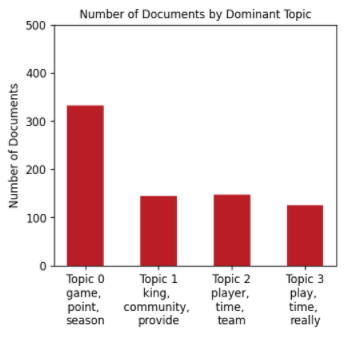
\includegraphics[width=3.4in]{figures/topic_doc_count.png}
	\caption[]{Topic Document Counts} 
	\label{counts} 
\end{figure}


Figure \ref{counts} and Table \ref{table_topic} show the distribution of documents classified by their dominant topic. 
The LDA topic model was able to keep a fairly equal number of articles in each topic.
This unsupervised learning model was able to avoid the issues of imbalanced, or skewed, distributions see in Activities 2 and 5.

\begin{table}[!htb] 
  \centering 
  \begin{tabular}{@{\small}lllll@{}} 
    \toprule % utilise booktabs
    & {\footnotesize Topic 1} &  {\footnotesize Topic 2} & {\footnotesize Topic 3} & {\footnotesize Topic 4} \\ \midrule
    Relevant & 192 & 10 & 30 & 43 \\
    Irrelevant & 140 & 135 & 119 & 82 \\
    Total & 332 & 145 & 149 & 125 \\
    \bottomrule
\end{tabular} \caption{NBA News Articles per topic. } \label{table_topic}
\end{table}

Topics 2 and 3 could be used to filter out irrelevant NBA news articles for a sports bettor. 
They contain 7\% and 20\% relevant articles for each topic and 3.6\% and 10.9\% of the total number of relevant documents in the corpus. 
Simply filtering out these two topics, the percentage of relevant articles in the corpus increases from 36.6\% to 51.4\%.



\subsubsection{Topic 1: Game Analysis}

The first topic created in the LDA modeling contained the majority of the articles that are relevant for a sports bettor.
This topic focuses on words that relate to pre-game and post-game analysis with words like "Game", "Point", "Score", and "Win".

The LDA model's equation for Topic 1 is:
\begin{align*}
    Topic\ 1 = 0.062*Game + 0.042*Point \\
    + 0.029*Season + 0.017*Score \\
    + 0.016*Rebound + 0.016*First \\
    + 0.016*Last + 0.015*Win \\
    + 0.014*Lead + 0.013*Team
    \label{eq:1}
\end{align*}

Figure \ref{weights1} is an interesting visual showing the weights of the most important terms used in this topic as well as the counts of those terms. 
Figure \ref{words1} contains a list of the top 30 words used within this topic.

\begin{figure}[!htb] \centering
	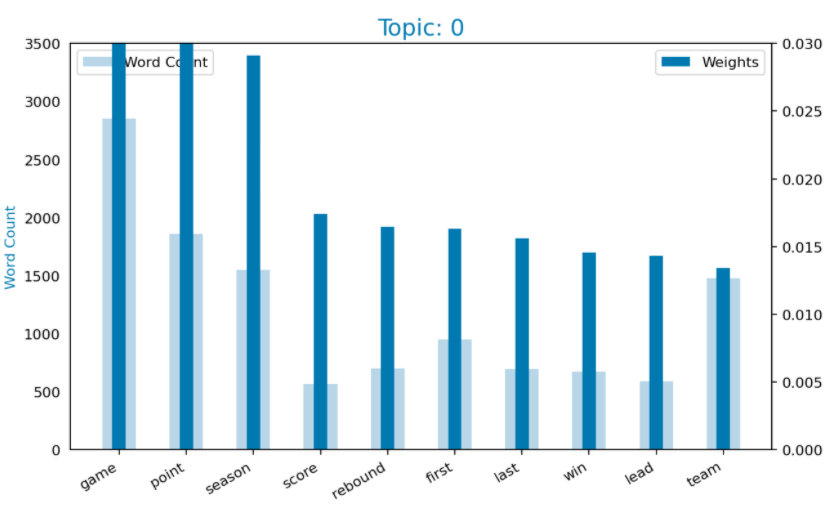
\includegraphics[width=3.4in]{figures/Topic0_words.png}
	\caption[]{Topic 1 Word Weights} 
	\label{weights1} 
\end{figure}

\begin{figure}[!htb] \centering
	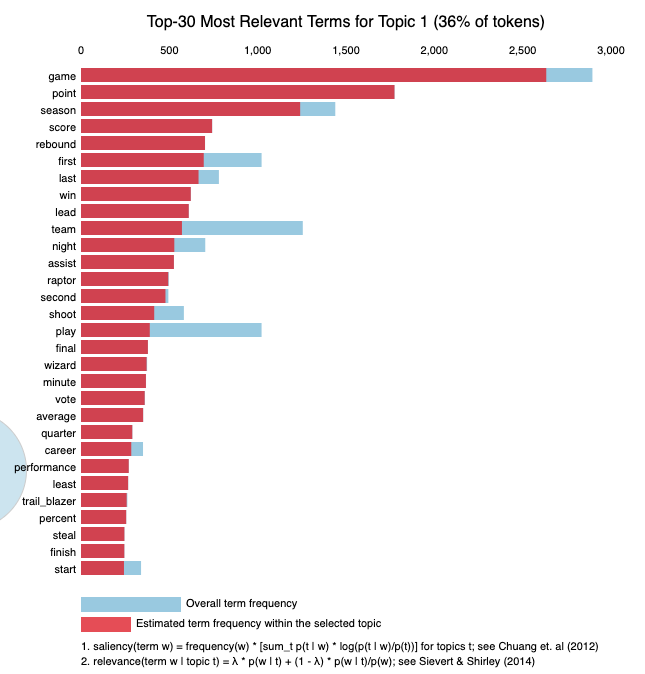
\includegraphics[width=3.4in]{figures/top_topic1.png}
	\caption[]{Top 30 words in Topic 1} 
	\label{words1} 
\end{figure}

\subsubsection{Topic 2: Community Service}


The second topic that was created focused almost entirely on news articles dealing with community outreach. 
This topic could be used to filter out the irrelevant NBA news articles for sports bettors.

The LDA model's equation for Topic 2 is:
\begin{align*}
    Topic\ 2 = 0.022*King + 0.018*Community \\
    + 0.014*Provide + 0.013*Support \\
    + 0.012*Help + 0.010*Create \\
    + 0.009*Team + 0.009*Local \\
    + 0.009*Work + 0.008*Effort 
    \label{eq:2}
\end{align*}

The NBA has a strong relationship with the communities the teams are in and these articles contained key words like "Family", "Community" "Provide" Support" "Help" "Local" "Team Work" or "Program". 
Figure \ref{words2} contains a list of the top 30 words used within this topic and Figure \ref{weights2} shows the weights associated with the top words. 

\begin{figure}[!htb] \centering
	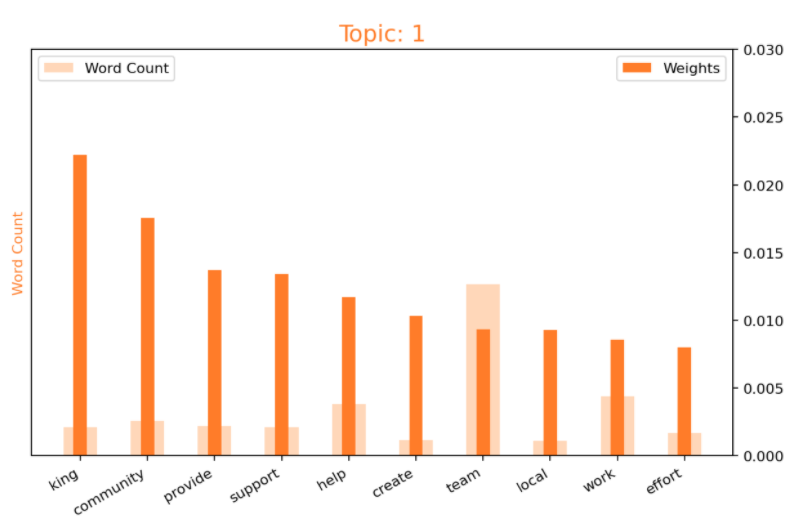
\includegraphics[width=3.4in]{figures/Topic1_words.png}
	\caption[]{Topic 2 Word Weights} 
	\label{weights2} 
\end{figure}


\begin{figure}[!htb] \centering
	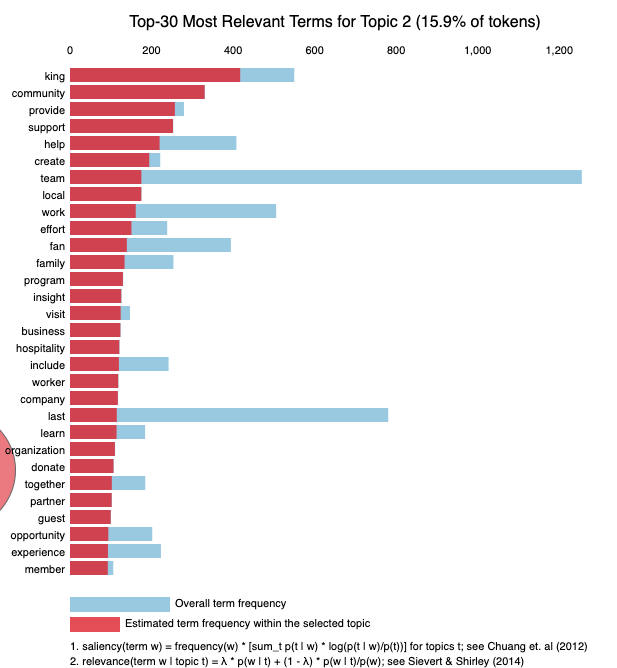
\includegraphics[width=3.4in]{figures/top_topic2.png}
	\caption[]{Top 30 words in Topic 2} 
	\label{words2} 
\end{figure}



\subsubsection{Topic 3: Player Focused}

Topic 3 is focused on players as people and not superstars. 
These articles discuss what the NBA players do outside of competing on the hardwood.

The LDA model's equation for Topic 3 is:
\begin{align*}
    Topic\ 3 = 0.021*Player + 0.015*Time \\
    + 0.014*Team + 0.014*Week \\
    + 0.012*Basketball + 0.011*Fan \\
    + 0.010*Ingle + 0.010*Burrell \\
    + 0.009*Life + 0.009*First
    \label{eq:3}
\end{align*}

Figure \ref{weights3} is an interesting visual showing the weights of the most important terms used in this topic as well as the counts of those terms. 

Figure \ref{words3} contains a list of the top 30 words used within this topic.


\begin{figure}[!htb] \centering
	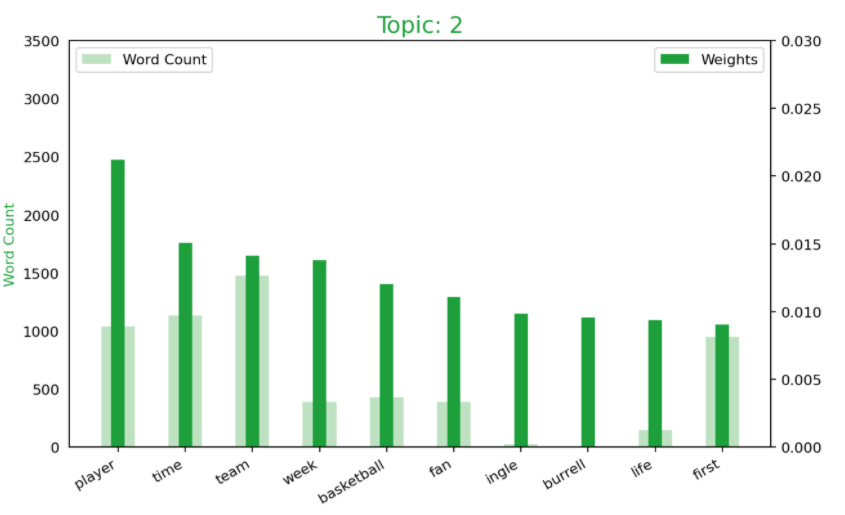
\includegraphics[width=3.4in]{figures/Topic2_words.png}
	\caption[]{Topic 3 Word Weights} 
	\label{weights3} 
\end{figure}

\begin{figure}[!htb] \centering
	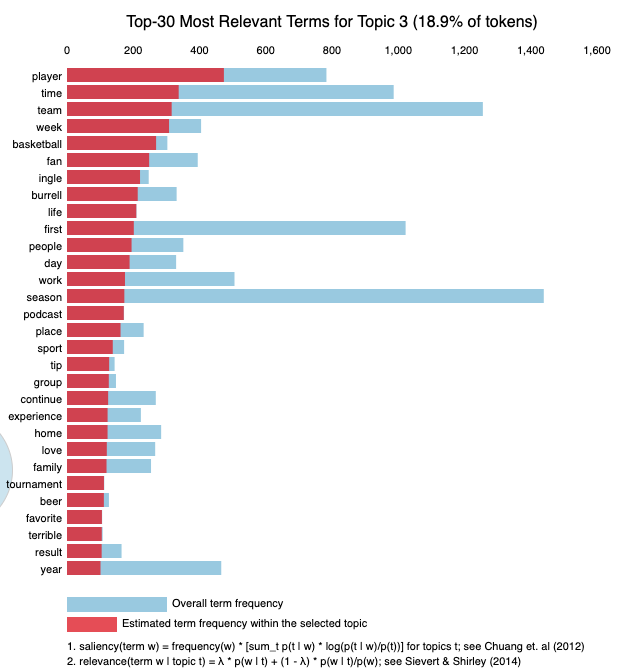
\includegraphics[width=3.4in]{figures/top_topic3.png}
	\caption[]{Top 30 words in Topic 3} 
	\label{words3} 
\end{figure}



\subsubsection{Topic 4: Covid Shutdown (looking back)}

This topic includes many of the miscellaneous articles, especially those written after the NBA shut down because of the Covid-19 virus.
This topic also includes many of the trade specific relevant articles.

The LDA model's equation for Topic 4 is:
\begin{align*}
    Topic\ 4 = 0.018*Play + 0.012*Time \\
    + 0.011*Really + 0.011*Great \\
    + 0.010*Thing + 0.010*Look \\
    + 0.010*Back + 0.010*Feel \\
    + 0.009*Well + 0.008*Bar
    \label{eq:4}
\end{align*}


Figure \ref{weights4} and Figure \ref{words4} provide graphs of the key terms used in this topic and their associated weights.


\begin{figure}[!htb] \centering
	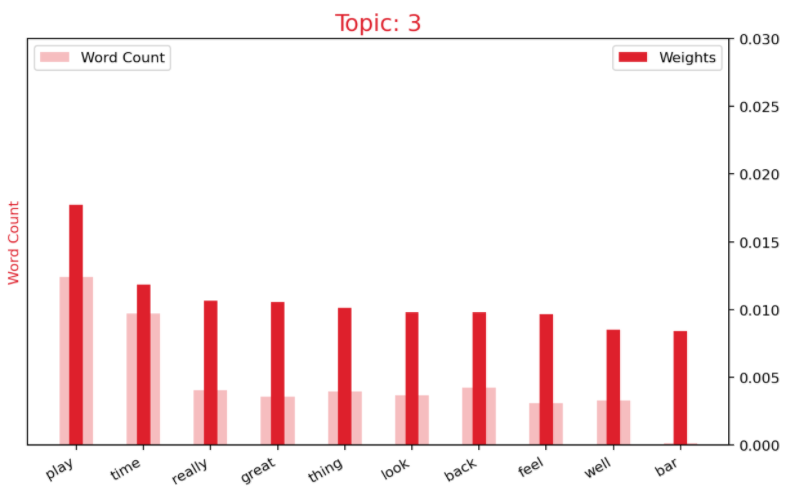
\includegraphics[width=3.4in]{figures/Topic3_words.png}
	\caption[]{Topic 4 Word Weights} 
	\label{weights4} 
\end{figure}


\begin{figure}[!htb] \centering
	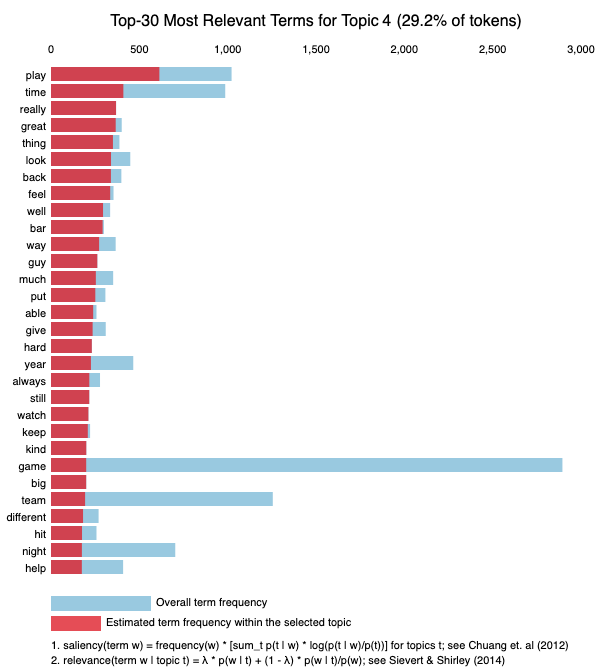
\includegraphics[width=3.4in]{figures/top_topic4.png}
	\caption[]{Top 30 words in Topic 4} 
	\label{words4} 
\end{figure}



\section{Discussion and Conclusions}

There are many benefits to using unsupervised machine learning techniques.
However, they can produce uncontrollable and often sub-optimal results depending on the data and the use case. 
For the purpose of a professional sports bettor overwhelmed with incoming news articles, the unsupervised machine learning methods of clustering and topic modeling performed worse than the document classification model built in the previous project \citep{project2}.

There is potential to achieve even more efficiency for a professional sports bettor by applying supervised learning methods and unsupervised learning methods in tandem. 
Future work could examine the accuracy and effectiveness of a data flow pipeline utilizing document filtering based on the supervised classification model followed by an unsupervised topic modeling algorithm to sort the remaining relevant news articles.
This flow may prove to be the optimal solution to the original problem posed in this and the previous NLP project that professional sports bettors face.

As for the unsupervised machine learning results, future work should include improvements to the pre-processing of the raw text data. 
For example, the clustering and topic modeling algorithms were erroneously creating divisions based on which team the news article was discussing. 
This is problematic and defeats the purpose of using these techniques owing to the knowledge that each article is tagged with the team based on which team website the article was scraped from. 

A potential solution could come by building off of the ontology in Activity 8 with raw terms grouped together at the given node from Figure \ref{Ontology}. 
Each team name mentioned in the articles could be grouped together into a single "NBA Team" term allowing for an anonymized term representing all teams to stop clusters from forming around a specific team.
This could also be extended to player names; a single term can be used to represent all NBA players. 
Depending on the situation, it may work better to have NBA players be represented by two terms, a term for the starting players on a team and a term for the bench players on a team. 

There were many lessons learned and extensions to future work that have been unearthed during this study.
This future work will need to be completed to better calibrate the document clustering models before A.I. Sports will be able to confidently implement the models as a product in the real sports betting world. 

In conclusion, while there needs to be more work to improve the results, this study was still able to accomplish the primary goal of using unsupervised machine learning techniques to better understand and organize the NBA news article corpus. 
Unsupervised learning algorithms provide a quick solution for understanding large quantities of text documents.
Valuable insights into the NBA news article corpus were gained both by using the documents as objects and by using the terms in each document as objects through this study. 


\clearpage


Appendix

\begin{figure}[!htb] \centering
	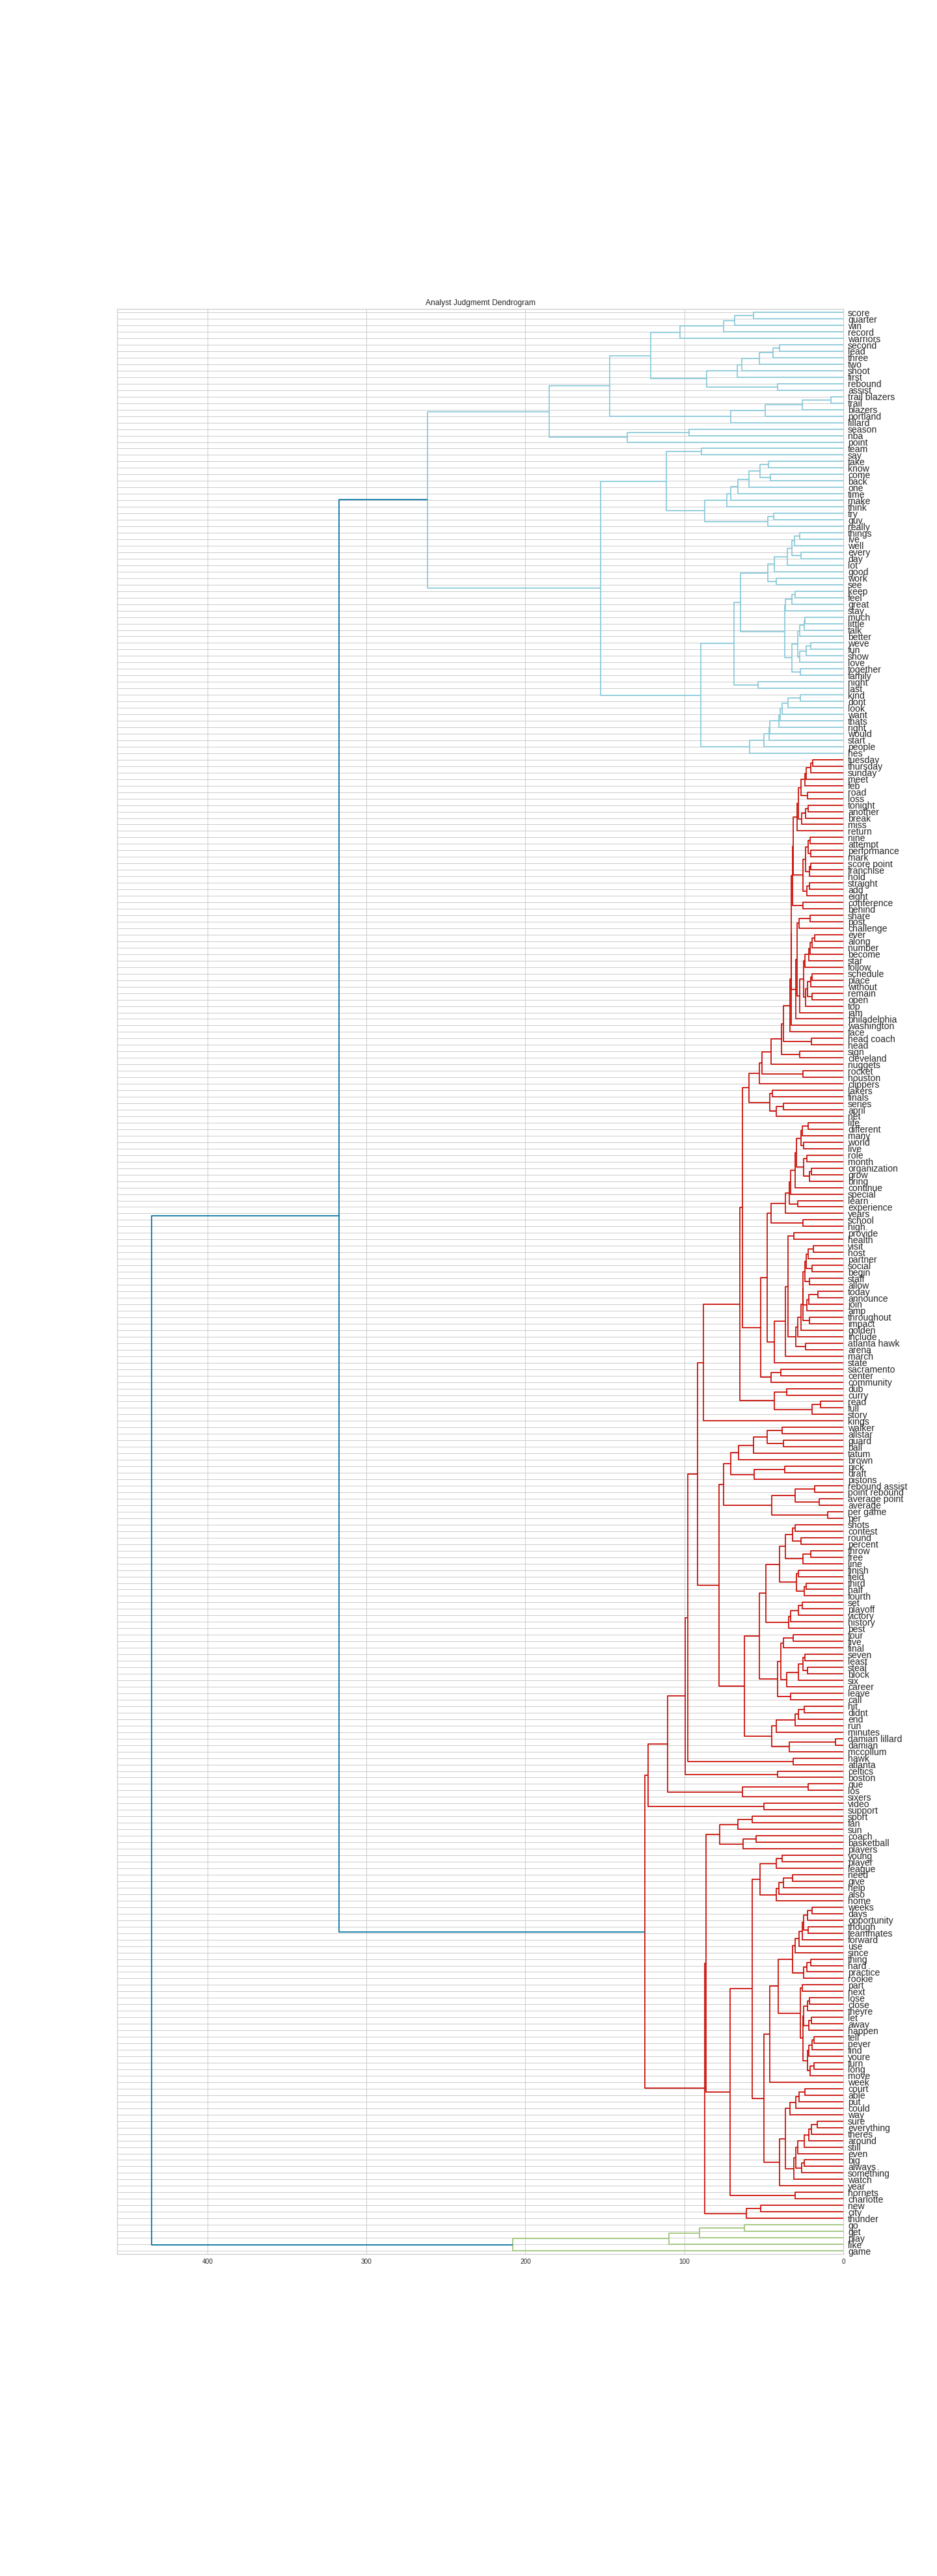
\includegraphics[width=3.4in]{figures/analyst_dendrogram.png}
	\caption[]{Analyst Dendrogram} 
	\label{AnalystDendrogram} 
\end{figure}

\begin{figure}[!htb] \centering
	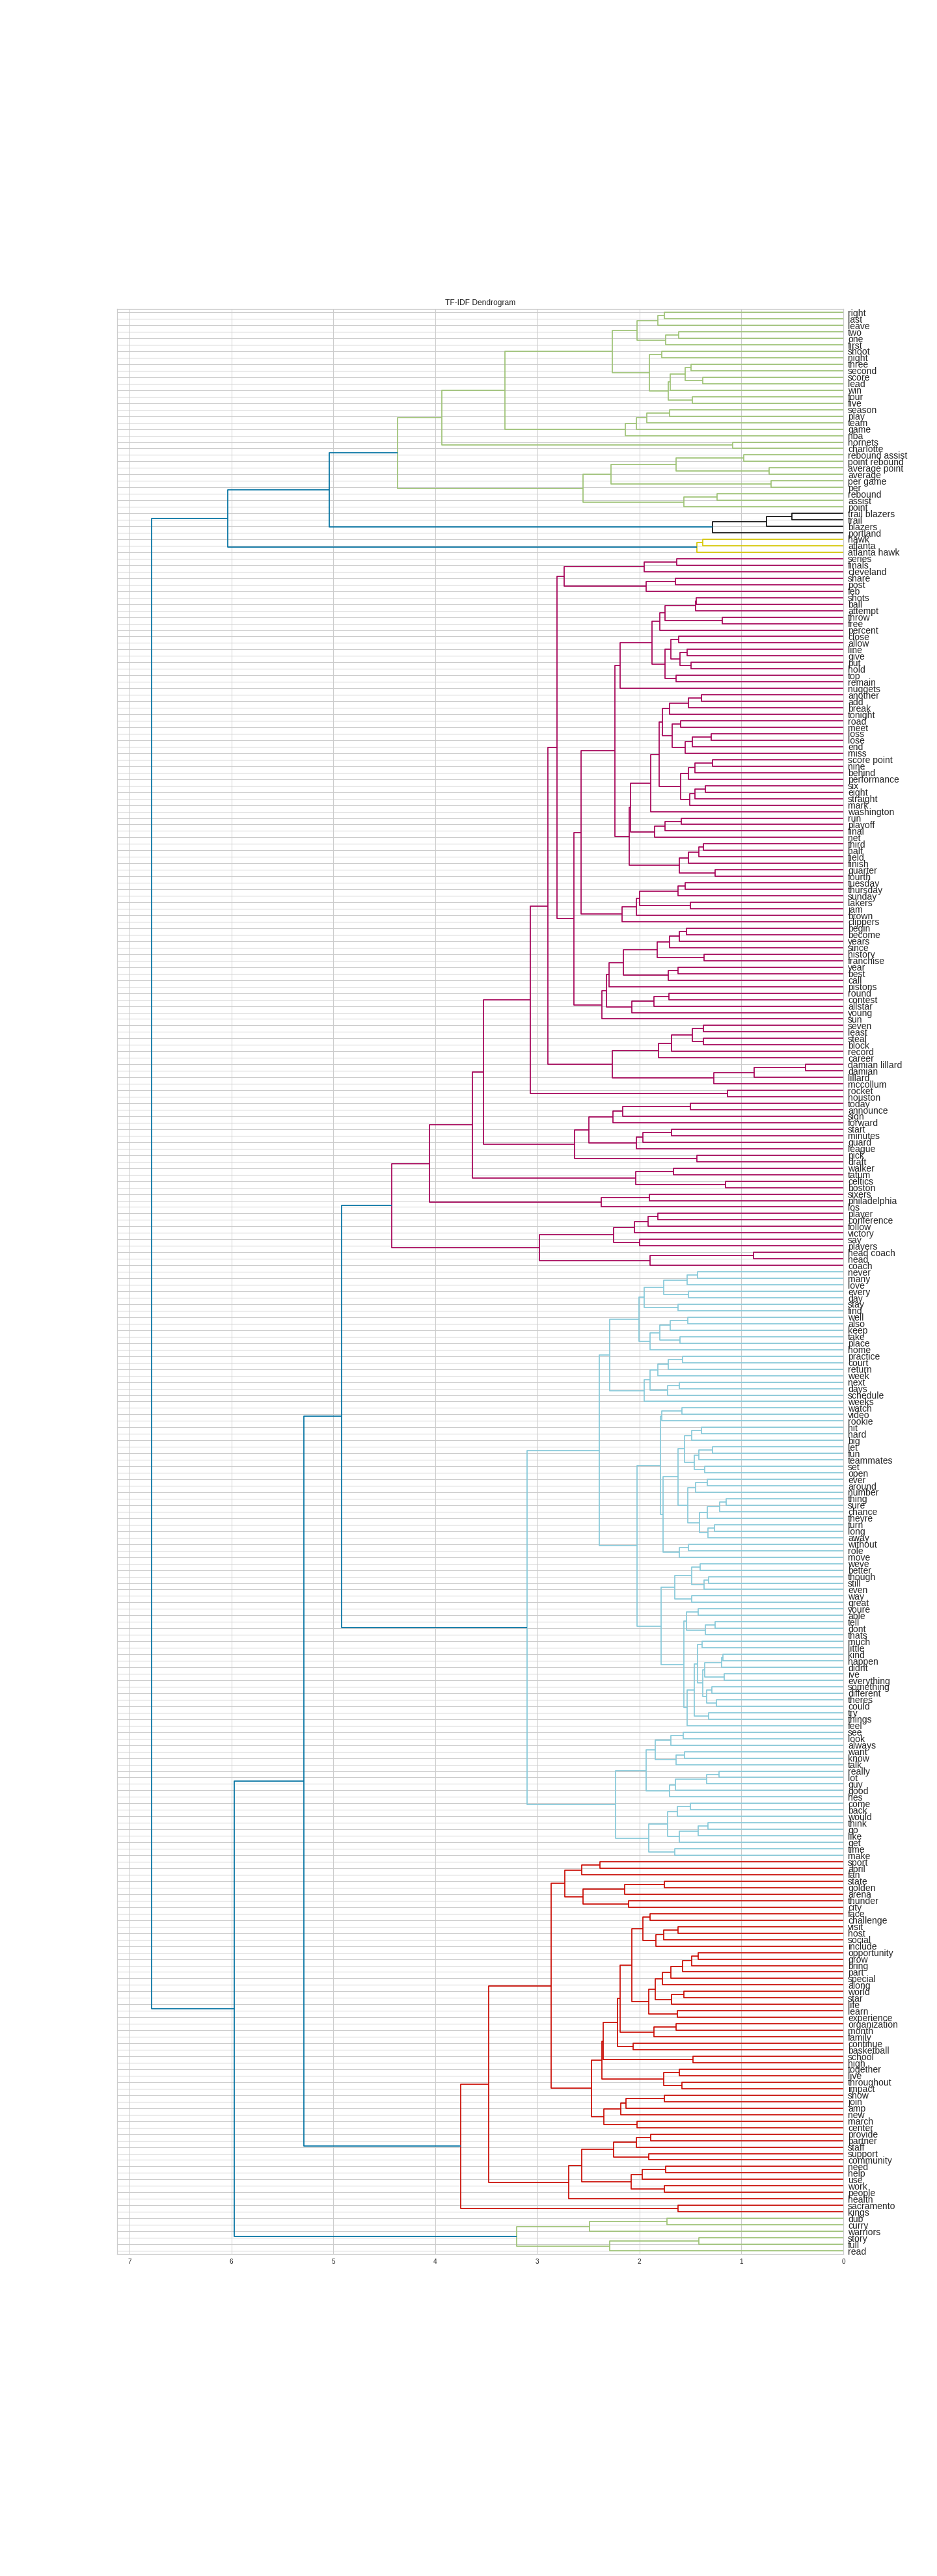
\includegraphics[width=3.4in]{figures/tfidf_dendrogram.png}
	\caption[]{TF-IDF Dendrogram} 
	\label{TF-IDFDendrogram} 
\end{figure}


\clearpage


\bibliography{bibliographie.bib}

\bibliographystyle{newapa}

\end{document}